% 1: Regular slides
%------------------
\documentclass[xcolor=svgnames,10pt]{beamer}

% 2:  Handouts
%------------------
%\documentclass[handout,xcolor=svgnames]{beamer}
%\usepackage{handoutWithNotes}
%\pgfpagesuselayout{4 on 1 with notes}[a4paper,border shrink=5mm]

% 3: Article style
%------------------
%\documentclass[a4]{article}
%\usepackage{beamerarticle}


%---- Begin PDF metadata ---------%
\usepackage{hyperref}
\hypersetup{%
	pdftitle={URDAD as Quality-Driven Process},%
	pdfauthor={Fritz Solms, Stefan Gruner and Cuen Edwards},%
	pdfsubject={},%
	pdfkeywords={URDAD, Quality driver}%
}
%---- End PDF metadata ---------%

% --- Graphics support ----%
\usepackage{graphicx}

% ---- Ticking clock for presentation ---%
% Duration of presentation = 20 minutes, change color at 50% and 80% of time, update clock every 29 seconds
% This is used in conjunction with \tdtime, \crono or \cronominutes
\usepackage[font=Times,timeinterval=29, timeduration=20.0, timedeath=0, fillcolorwarningsecond=white!60!yellow,timewarningfirst=50,timewarningsecond=80]{tdclock}


%--------------- Begin Beamer styling  -------------%

\usetheme{Berkeley}
% default 
%	AnnArbor | Antibes | Bergen |
%	Berkeley | Berlin | Boadilla |
%	boxes | CambridgeUS | Copenhagen |
%	Darmstadt | default | Dresden |
%	Frankfurt | Goettingen |Hannover |
%	Ilmenau | JuanLesPins | Luebeck |
%	Madrid | Malmoe | Marburg |
%	Montpellier | PaloAlto | Pittsburgh |
%	Rochester | Singapore | Szeged |
%	Warsaw

\setbeamertemplate{background canvas}{
\includegraphics
	[width=\paperwidth,height=\paperheight]{background.png}}
\setbeamercolor{structure}{fg=DarkSlateGray} 
\setbeamercolor{normal text}{fg=Black} 
%\setbeamercolor{alerted text}{fg=Crimson} 
%\setbeamercolor{alerted text}{fg=DarkRed} 
\setbeamerfont{structure}{series=\bfseries} 
%\setbeamersize{text margin left=10mm}

% To insert outline slides before every section
%\AtBeginSection[]
%{
%   \begin{frame}
%       \frametitle{Outline}
%       \tableofcontents[currentsection]
%   \end{frame}
%}

%--------------- End Beamer styling  -------------%

\usepackage{color}
\usepackage{listings}
\lstdefinelanguage{urdad}
{
keywords=
  {Model,ResponsibilityDomain,Query,Constraint,QualityConstraint,FunctionalRequirements,receiving,yielding,
  StateConstraint,stateAssessmentProcess,InverseConstraint,inverseOf,AndConstraint,AND,OrConstraint,OR,
  XorConstraint,XOR,from,to,many,BasicDataType,DataStructure,is,abstract,has,Variable,ofType,Constant,
  ValueOf,Exception,attribute,identification,identifying,association,linking,aggregate,component,
  QualityRequirement,requiredBy,constraint,with,constructedUsing,ResultConstraint,PreCondition,
  raises,checks,PostCondition,ensures,use,toAddress,if,ServiceContract,undoneUsing,Request,Result,
  Service,realizes,doSequential,choice,else,doConcurrent,blocking,Concurrency,wait,until,create,set,
  equalTo,add,remove,requestService,on,raiseException,returnResult,while,do,forAll,Note},%
sensitive=true,%
alsoletter={\$},%
comment=[l]{\#},%
string=[b]",%
string=[b]'%
}

%\definecolor{OliveGreen}{cmyk}{0.64,0,0.95,0.40}
%\definecolor{CadetBlue}{cmyk}{0.62,0.57,0.23,0}
\definecolor{lightgray}{gray}{0.9}
\lstset{
language=urdad,  
basicstyle=\ttfamily\tiny,
keywordstyle=\itshape\color{blue},
%keywordstyle=\color{blue},        % Keywords font ('*' = uppercase)
commentstyle=\color{gray},           
numbers=left,                           % Line nums position
numberstyle=\tiny,                      % Line-numbers fonts
stepnumber=1,                           % Step between two line-numbers
numbersep=5pt,                          % How far are line-numbers from code
backgroundcolor=\color{lightgray}, % Choose background color
frame=none,                             % A frame around the code
tabsize=2,                              % Default tab size
captionpos=b,                           % Caption-position = bottom
breaklines=true,                        % Automatic line breaking?
breakatwhitespace=false,                % Automatic breaks only at whitespace?
showspaces=false,                       % Dont make spaces visible
showtabs=false,                         % Dont make tabls visible
columns=flexible,                       % Column format
%morekeywords={__global__, __device__},  % CUDA specific keywords
}


\usepackage{color}
\usepackage{listings}
\lstdefinelanguage{pseudoCode}
{
keywords=
  {class,public,for,while,if,try,catch,return},%
sensitive=true,%
alsoletter={\$},%
comment=[l]{\#},%
string=[b]",%
string=[b]'%
}

%\definecolor{OliveGreen}{cmyk}{0.64,0,0.95,0.40}
%\definecolor{CadetBlue}{cmyk}{0.62,0.57,0.23,0}
\definecolor{lightgray}{gray}{0.9}
\lstset{
language=pseudoCode,  
basicstyle=\ttfamily\footnotesize,
keywordstyle=\itshape\color{blue},
%keywordstyle=\color{blue},        % Keywords font ('*' = uppercase)
commentstyle=\color{gray},           
numbers=left,                           % Line nums position
numberstyle=\tiny,                      % Line-numbers fonts
stepnumber=1,                           % Step between two line-numbers
numbersep=5pt,                          % How far are line-numbers from code
backgroundcolor=\color{lightgray}, % Choose background color
frame=none,                             % A frame around the code
tabsize=2,                              % Default tab size
captionpos=b,                           % Caption-position = bottom
breaklines=true,                        % Automatic line breaking?
breakatwhitespace=false,                % Automatic breaks only at whitespace?
showspaces=false,                       % Dont make spaces visible
showtabs=false,                         % Dont make tabls visible
columns=flexible,                       % Column format
%morekeywords={__global__, __device__},  % CUDA specific keywords
}

%---------------------------------------------------%

\title[URDAD as Quality-Driven Process]{URDAD as Quality-Driven Process
\footnote{Accepted as a regular paper at SOMET 2011, the 10 International Conference on Intelligent Software Methodologies, Tools, and Techniques, St Petersburg, 28 - 30 Sept 2011}}

\author[Solms,Gruner,\\Edwards \\ \ \\ \cronominutes \\ \ \\]{Fritz Solms, Stefan Gruner and Cuen Edwards}

\institute[Univ Pta]{
  URDAD-MDE subgroup of SSFM \\
  Department of Computer Science\\
  University Of Pretoria\\[1ex]
  \texttt{fritz@solms.co.za}
}

\date[June 2011]{June 9, 2011}
%\date{\tddate \ \ \tdtime}

\begin{document}

  \maketitle

  \section{Background}

\begin{frame}{Background}
  \begin{itemize} 
    \item<+-| alert@+> Inferior requirements
      \begin{itemize}
      \item Core contributor to poor software quality \& high cost.
      \end{itemize}
    \item<+-| alert@+> Formal methods
      \begin{itemize}
      \item Use mathematical modeling \& formal logic to to specify \& verify requirements.
      \item However, incur high cost \& skills requirements.
      \end{itemize}
    \item<+-| alert@+> Semi-formal methods
      \begin{itemize}
	\item Constrain cost \& skills requirements.
	\item Formalization of process \& inputs/outputs.
	  \note[item]{Main complexity in constraint specification.}
    
      \end{itemize}
  \end{itemize}
\end{frame}



  \section{Definitions}

\begin{frame}{Definitions}

\alert<1>{
  \begin{definition}
   \emph{Quality} is the degree to which a set of inherent characteristics fulfills requirements.
	 \footnote{David Hoyle, {\em {ISO} 9000: 2000 Quality Systems Handbook}. 4th ed, 2000.}
  \end{definition}}
    \pause

\alert<2>{
  \begin{definition}
   A \emph{quality criterion} is an observable quality characteristic of the solution.
  \end{definition}}
    \pause

\alert<3>{
  \begin{definition}
   A \emph{quality measure} is a quantitative metric for a quality criterion.
  \end{definition}}
    \pause

\alert<4>{
  \begin{definition}
	 	 A \emph{quality driver} is an activity which improves one or more process or model quality criteria.
	 \footnote{P.~G Petersen, et al., Software quality drivers and indicators. {\em System Sciences}, p210 --218 vol.2, 1989.}
  \end{definition}}
\end{frame}

  \begin{abstract}
Use-Case Responsibility-Driven Analysis and Design (URDAD) is a service-oriented software analysis and design methodology. It is used by requirements engineers to develop technology-neutral, semi-formal platform-indepen\-dent models (PIM) within the OMG's MDA. In the past, URDAD models were denoted in UML. However, that was tedious and error-prone. The resulting models were often of rather poor quality. In this paper we introduce and discuss a new Domain-Specific Language (DSL) for URDAD. Its meta model is consistent and satisfiable. We show that URDAD DSL specifications are simpler and allow for more complete service contract specifications than their corresponding UML expressions. They also enable traceability and test case generation.
\end{abstract}


  \section{URDAD}

\begin{itemize}
  \item Modeling in problem domain
  \item sevices-oriented analysis and design methodology
  \item contract focused
  \item Responsibility driven
  \item semi-formal (agile/formal)
  \item levels of granularity
  \item
\end{itemize}


%  \subsection{Quality requirements}

In order to be able to measure quality, we need to identify the quality requirements. Requirements only make sense from the perspective of the stakeholder who requires the requirment. Hence to identify quality requirements we need to first identify the stakeholders who have an interest in the process as well as those who have an interest in the resultant analysis and design model. Once we have identified the stakeholders, we can elicit the quality requirements

We differentiate between quality requirements for the process itself from the quality requirements on the outputs (the analysis and design model).

\cite{berard_what_1995}

Stake holders:
\begin{itemize}
  \item Project management (measurability, repeatability, estimatability)
  \item Requirements specialists (ease of use, simple process, defined process activities, defined inputs and outputs, tool support)
  \item Business (low cost, trainable, grow in islands)
\end{itemize}


\begin{itemize}
  \item Process measurability
  \item Repeatability
  \item Defined inputs and outputs
  \item Clearly specified tasks with defined activities
  \item Process consistency (URDAD generates itself)
\end{itemize}

Can apply process to a sub-world, decouples from higher and lower level granularities via contracts

Could introduce more abstract qualities and things the process must have to realize these, e.g. \emph{usability} affected by many of these

CMM requires process definition


\subsection{Internal process consistency}

Here show that if you use URDAD to design an analysis and design methodlogy, you will get URDAD. Feed additional concepts into URDAD.

Here identify the stakeholders in both, the process and the outputs of the process and their quality requirements.

  \section{Quality drivers}
\label{sec:qualityDrivers}

A quality drivers is defined as an activity which improves one or more process or model quality criteria\cite{petersen_software_1989}. The relience on quality-drivers forms the basis for the concept of a \emph{`quality-driven'} process. In this section we look at each model and process quality criterion and discuss activities (quality drivers) which can be used to improve the quality criterion. The list of quality-drivers presented here is not intended to be exhaustive but includesrepresents a collection of quality-drivers which are widely known and used. In addition to identifying quality-drivers, we also note that quality metrics can be applied to the resultant model in order to assess model quality. This section discusses some commonly used quality metrics for the identified quality criteria suitable for a service-oriented approach. For a more general list of model quality metrics the reader should consult \cite{mohagheghi_existing_2009}.

\subsection{Model quality drivers}

\emph{Semantic Model Quality} relates to semantic accuracy and completeness. It is influenced by the quality of the modeling language and hence by the semantic quality of the metamodel of the modeling language. The latter is determined by its semantic completeness, consistency and complexity\cite{buder_effects_2010}. Semantic completeness refers to the power of the formal language to express all propositions. More precisesly, a formal system is said to be semantically complete if and only if every theorem of the system is provable in the system.  A core semantic quality-driver is thus the specification of a metamodel for the analysis and design model which itself is shown to be semantically complete and consistent.

\emph{Syntactic Quality} elates to correct language usage\cite{lange_christiaan_assessing_2007}, i.e.\ that the grammatical statements made comply to the abstract syntax as specified via the metamodel and its constraints or an ontology and its associated rules. A commonly used syntactic quality driver is the definition of concrete text and/or graphical grammars and a transformation between the concrete and abstract syntax. Models which are defined through and verified against the concrete syntax can be shown to comply to the abstract syntax of the associated metamodel. Editors generated from the concrete syntax definition generally validate syntactic correctness. In this paper we confine the assessment of syntactic quality to the existence of a formal modeling language and concrete grammar for model specification. We will thus assume that model instances will adhere to the grammar of the chosen modeling language as this can easily be verified.

\emph{Simplicity} is the inverse of complexity. The complexity of the modeling language is usually assessed by measuring the complexity of the metamodel for that language\cite{mohagheghi_evaluating_2007}. A lot of work has been done on model complexity itself. Common approaches include using information entropy measures\cite{abrahamsson_extreme_2004}, language-theoretic approaches\cite{podgorelec_estimating_2007} and function complexity assessment based on the McCabe complexity measure \cite{mccabe_complexity_1976}. A service-oriented approach already enforces certain drivers for simplicity. In particular it enforces the assembling of functions from independent, stateless services, the enforced decoupling through services contracts, the improved reuse through the implied service discovery, as well as an implied adapter layer facilitating reuse across technologies and interfaces mismatches. A metamodel confining the modeling constructs and relationships between these, as well as a convenient grammar, reduce complexity. Another core driver for simplicity is the decomposition across levels of granularity enabling the understanding and processing of one level of granularity before having to concern oneself with the details of the next lower level of granularity. The availability of a services contract enables one to look at a service from a user/service consumer perspective before understanding the service function. Finally, traceability links and in particular enforced satisfaction links (i.e.\ that a functions may only use services which address functional requirements of the service) are drivers for simplicity.

\emph{Completeness} of requirements is difficult to assess, though the discovery of certain stakeholders for which no functional or non-functional requirements exist is an indication of missing requirements. Design completeness is easier to assess as there is a global point of reference - the degree to which the requirements are fulfilled. Core quality-drivers for completeness include enforced satisfaction links, the enforcement of testable pre- and post-conditions, as well as having a metamodel which enforces certain content, either structurally, or through metamodel constraints. In a service-oriented approach, a completeness metric can be specified as a function of 1) the percentage of functional requirements not addressed in the designed functions (identified through missing satisfaction links)\cite{shim_design_2008}, 2) the fraction of pre- and post-conditions for which the test process has not been specified and 3) the percentage of request and result classes for which the data structures have not been specified. At the implementation level completeness can be assessed as the fraction of services for which service implementations are not yet available.

\emph{Consistency} is an important model property. A lot of emphasis has been placed on model consistency for UML models. This is so because UML models are often inconsistent due to the multi-diagram approach and the complexity of the modeling language itself\cite{lange_empirical_2004}. A commonly quality-driver for model consistency is to use a much smaller (less general) language with more formally defined semantics which enforces the consistency through both, its structure and a set of metamodel constraints.

\emph{Cohesion} in a service-oriented approach has been extensively studied by Mikhael Perepletchikov et al.\ \cite{perepletchikov_cohesion_2007,perepletchikov_impact_2010}. Their approach is closely related to that of unity criteria \cite{gonzalez_unity_2009} identifying and quantifying interfacing cohesion, usage cohesion and implementation cohesion. These cohesion measures can be applied directly to an URDAD model. Quality-drivers for cohesion include enforcing the single responsibility principle as well as localizing all controll and decision logic for a service in a controller service. 

\emph{Decoupling} is enforced in a service-oriented approach by requiring that services are only consumed via services contracts. This decouples services across levels of granularity. Quality-drivers for decoupling include a metamodel which enforces contracts based decoupling through metamodel structure and localization of function logic within a controller. The latter ensures that lower level services remain decoupled, i.e.\ that they do not call each other. In a service-oriented architecture, the number of services which are directly coupled to concrete lower level services can be used as a measure of coupling\cite{shim_design_2008}.

\emph{Modifiability} refers to the efficiency with which model changes can be applied, i.e.\ it is related to the inverse of the cost required to make model changes. Modifiability is difficult to quantitatively measure. It is supported by other model qualities like \emph{simplicity},  \emph{decoupling} (modifiability through pluggability), and \emph{cohesion} (localized maintenance). A further quality-driver in the form of localizing function logic within a controller service, thereby projecting out additional levels of granularity. Shim et al.\ \cite{shim_design_2008} define a quality metric for modifiability (flexibility) of service-oriented designs as a weighted sum of coupling, service granularity, and parameter granularity. Since increased complexity and coupling reduce modifiability, the quality drivers for simplicity and decoupling are also quality drivers for modifiability.

\emph{Reusability} provides a measure of the ability and likelihood that a service can be reused. Khoshkbarforoushha et al.\  \cite{khoshkbarforoushha_metric_2010,choi_quality_2008,feuerlicht_determinants_2007}
\cite{khoshkbarforoushha_metric_2010} point out that service reusability is often caused by contract and requirements mismatch. The former can be addressed via adapters. Core quality-drivers for reusability include \emph{decoupling} via services contracts with the latter also driving discoverability and consumability, \emph{levels of granularity} via process localization within a reusable controller service, and \emph{cohesion} through enforcing the single responsibility principle. Indeed, \cite{shim_design_2008} defines a simple quantitative reusability measure for service-oriented systems as a weighted sum of coupling, cohesion, granularity, and consumability.

\emph{Traceability} is needed for design validation and estimation. Validation includes assessing sufficiency and necessity. Ramesh and Jarke \cite{ramesh_toward_2001} identify four types of traceability links in models including \emph{satisfaction} links used to assess whether requirements are satisfied, \emph{evolutionary} links to trace along the evolution of an artifact over time, \emph{rationale} links which typically link requirements to higher level business goals, and \emph{dependency} links enabling one to identify dependencies of model elements. Quality-drivers include thus the availability of these traceability links in the modeling language and their enforced usage through the modeling process.

  \section{Internal consistency of the URDAD methodology}
\label{sec:urdadConsistency}

URDAD is an analysis and design methodology used to design services. If one uses the methodology to design a service for analyzing the services contract and designing a technology neutral process for a service, the constructed model should be a model for URDAD, containing the URDAD process as the service process and the URDAD metamodel for the domain concepts. If this is not the case then URDAD would be inconsistent because it would state ``use this methodology to design services, but use something else/better to design the service for designing a service''.
      \begin{itemize}
		  \item Apply process to design service of performing analysis \& design for service.
			 \begin{itemize}
				\item Should result in service with process, semantics \& model structure which represents URDAD itself.
				\item If it doesn't, then not internally consistent.
            \item If it does, it does not show that URDAD is a good methodology, but only that it is consistent.
In order to validate the internal consistency of the URDAD methodology, we used URDAD to design the service of performing a services-oriented analysis and design. If the methodology is consistent it needs to either regenerate itself or at least something which is largely equivalent to itself. It would, of course, not follow that URDAD is a ``good'' methodology, only that it is a consistent methodology.

Due to space constraints we cannot go through the full process across levels of granularity. Instead we demonstrate the consistency by looking at a particular level of granularity and point out how URDAD starts regenerating itself as process and how its own metamodel is regenerated. We also use this opportunity to show aspects of the URDAD metamodel and the text grammar of the URDAD-DSL\footnote{A separate paper discussing the URDAD metamodel and domain specific language for URDAD is currently being reviewed.}. To make this more interesting we omit the first level of granularity which is a process which contains the analysis and process design steps for a particular level of granularity. We zoom directly into the \emph{performAnalysis} service which has more interesting pre- and post-conditions and consequently a more interesting process specification.

\begin{figure}[Htbp]
  \centering
  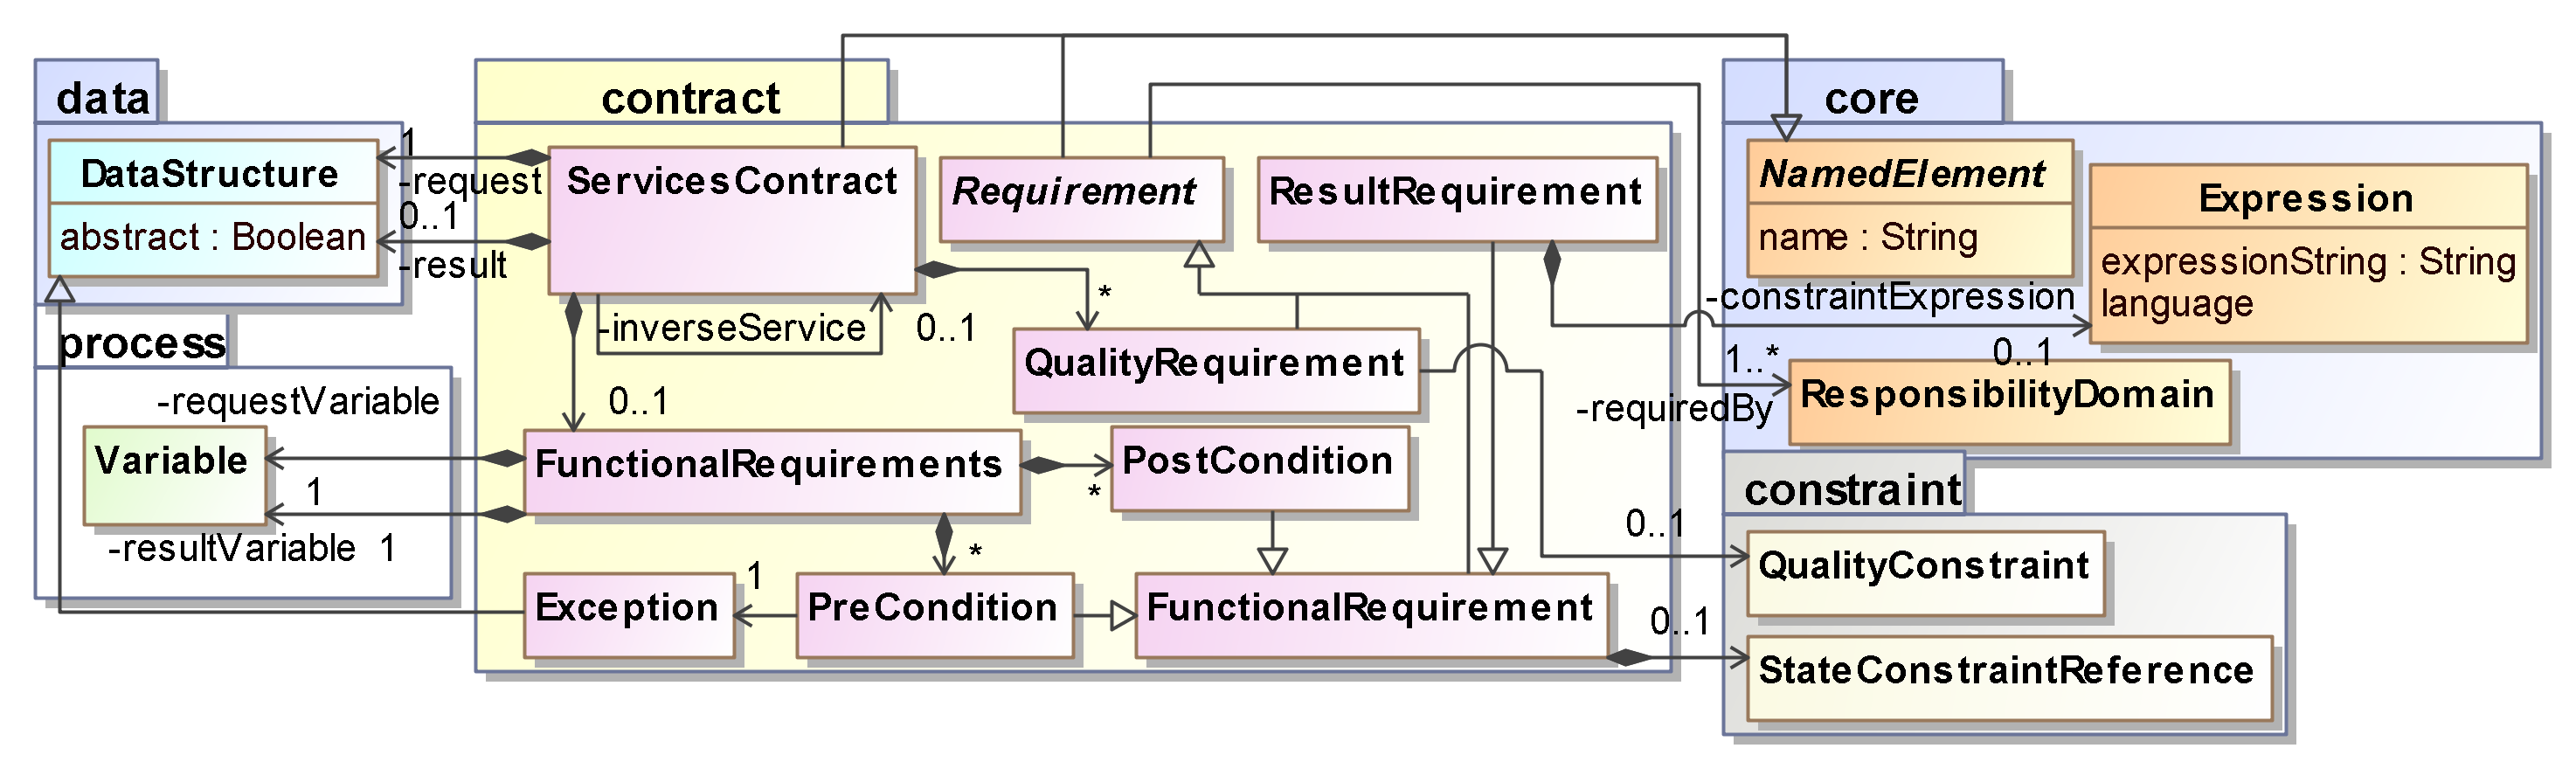
\includegraphics{contract}
  \caption{The modeling constructs available in URDAD introducing the semantics for services contracts}
  \label{fig:contractModule}
\end{figure}

We start by eliciting the stakeholders (yielding the stakeholders identified in section \ref{sec:qualityCriteria}) and their functional requirements. The output is a service contract specification for the \emph{performAnalysis} service which itself contains the concept of a service contract. The URDAD metamodel support for service contract specification is shown in figure \ref{fig:contractModule}. Below we use the text grammar defined for the URDAD-DSL to specify the service contract for the \emph{performAnalysis} service:

\lstset{language=urdad,caption=Specifying a state constraint in the URDAD text grammar.,label=contractTextSyntax}
\begin{lstlisting}[numbers=left,escapechar=|]

ResponsibilityDomain RequirementsEngineering
{
  ServiceContract provideService
  {
    FunctionalRequirements receiving Variable provideServiceRequest ofType ProvideServiceRequest yielding Variable provideServiceResult ofType ProvideServiceResult
    {
      PreCondition serviceHasStakeholders requiredBy (Client) raises NoStakeholdersException checks Constraint ServiceHasStakeholders
      PreCondition stakeholderRequirementsConsistent requiredBy (Client Implementation Testing) raises InconsistentStakeholderRequirementsException checks Constraint RequirementsConsistent
      PostCondition serviceContractSpecified requiredBy (Implementation Testing) ensures Constraint ServiceContractSpecified
      PostCondition serviceSourcedFromEnvironment if Constraint ServiceAvailable requiredBy (Client) ensures Constraint ServiceSourced with Query OCL:"serviceContract"
      PostCondition serviceSpecified if Constraint Not ServiceAvailable requiredBy(Client Implementation) ensures ServiceSpecified
      QualityRequirement traceability requiredBy (ProcessDesign ProjectManagement Development)  
    }
    Request DataStructure ProvideServiceRequest
    {
       has Component serviceRequirements ofType _ServiceRequirements
    }
    Result DataStructure ProvideServiceResult
    {
      has Component serviceContract ofType _ServiceContract
      has Component service ofType _Service
    }        
  }
  ...
} 
\end{lstlisting}

Note how we are already regenerating the URDAD metamodel in that the \verb+ServiceContract+ for perform analysis generates a domain which includes the concept of a \verb+_ServiceContract+. As we follow the URDAD methodology to design itself, we traverse levels of granularity, incrementally generating lower level aspects of the URDAD process and the URDAD metamodel, populating the finer details in the metamodel classes and the lower level process elements of the URDAD process. Throughout the classes without underscore prefix are the metamodel classes whilst the classes with underscore prefix are the classes generated by the methodology itself. 

\lstset{language=urdad,caption=Regenerated metamodel classes.,label=constraintTextSyntax}
\begin{lstlisting}[numbers=left,escapechar=|]
DataStructure _ServiceContract 
{
    has Component functionalRequirements ofType _FunctionalRequirements
    has Component request ofType _DataStructure
    has Component result ofType _DataStructure
}
\end{lstlisting}

\begin{figure}[Htbp]
  \centering
  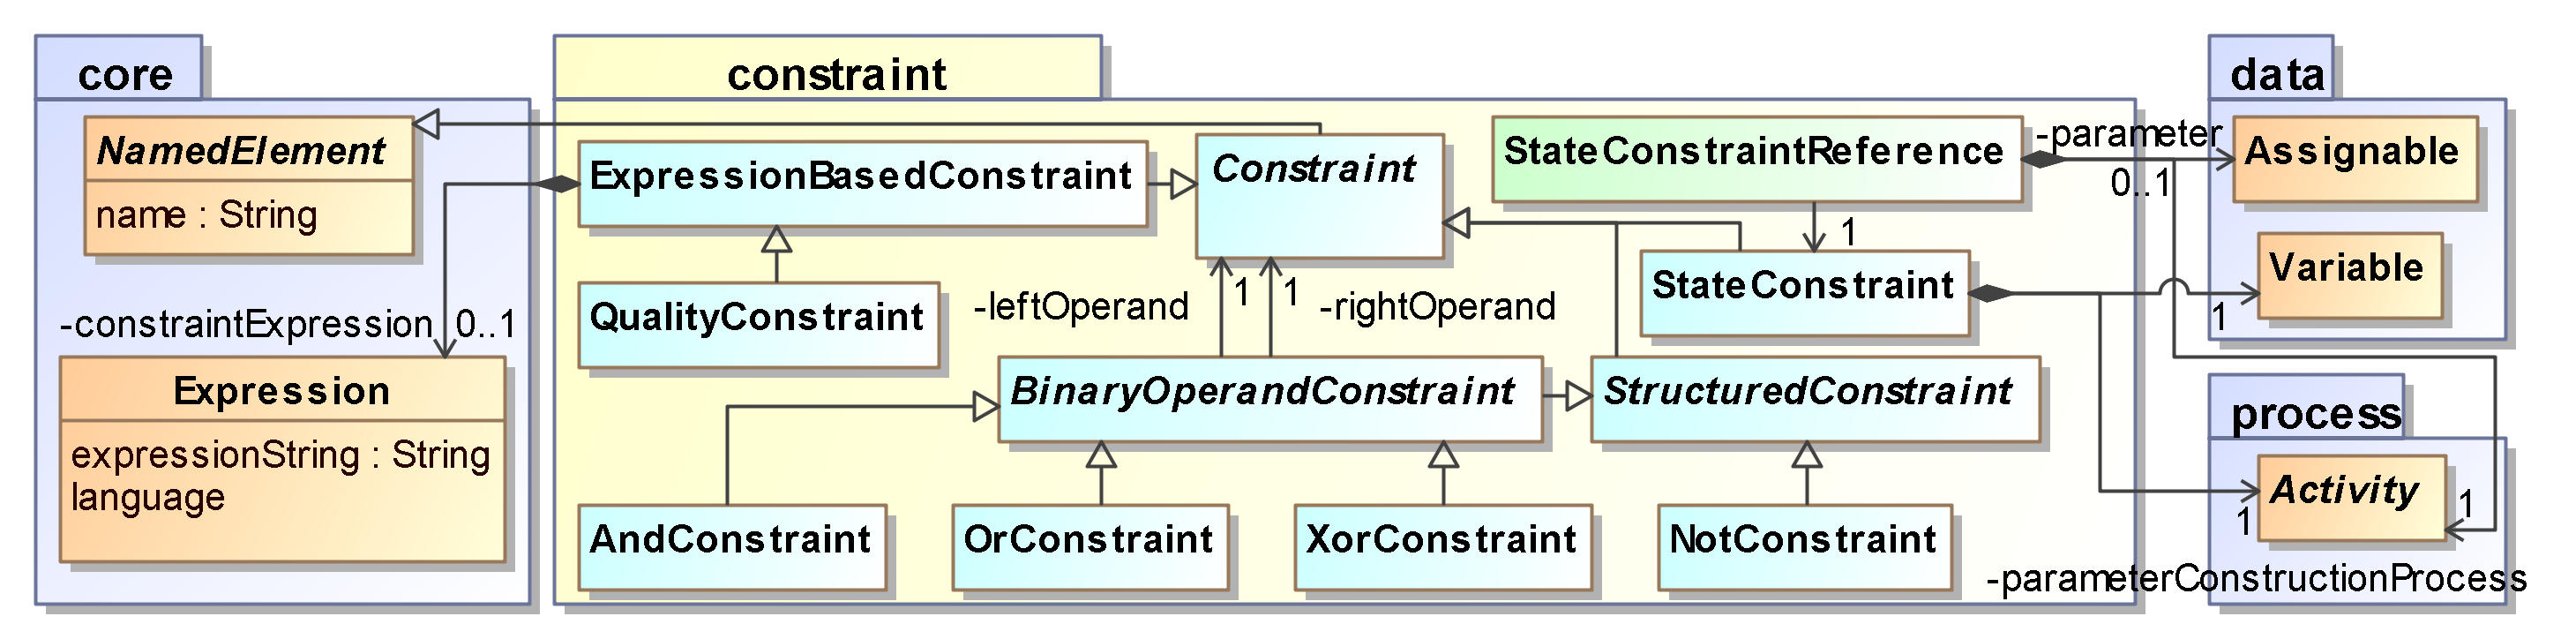
\includegraphics{constraint}
  \caption{The modeling constructs available in URDAD facilitating the specification of constraints.}
  \label{fig:constraintModule}
\end{figure}

Service contracts refers to reusable, parametrized state constraints. Figure \ref{fig:constraintModule}, shows URDAD's modeling elements for specifying such constraints. In a separate paper currently under review we have pointed out that the Object-Constraint Language (OCL)\cite{_object_2010}  alone is not expressive enough to specify reusable, parametrized constraints for a services oriented approach where one needs to extract information from the environment via services and then apply data structure constraints on the obtained environmental information.

The following listing shows an simple example of a parametrized constraint, \emph{ServiceHasStakeholders}, which demonstrated that a state constraint is assembled from a process that extracts information from the environment and a set of data constraints applied to the obtained information.
\lstset{language=urdad,caption=Specifying a state constraint in the URDAD text grammar.,label=processTextSyntax}
\begin{lstlisting}[numbers=left,escapechar=|]
StateConstraint ServiceHasStakeholders receiving Variable serviceRequirements ofType _ServiceRequirements 
{
  StateAssessmentProcess doSequential 
  {
    create Variable identifyStakeholdersRequest ofType IdentifyStakeholdersRequest
    set Query OCL:"identifyStakeholdersRequest.serviceRequirements" equalTo Query OCL:"serviceRequirements"
    requestService identifyStakeholders with identifyStakeholdersRequest yielding Variable identifyStakeholdersResult ofType IdentifyStakeholdersResult
  }
  Constraint OCL:"identifyStakeholdersResult->size() > 0"
}
\end{lstlisting}

\begin{figure}[Htbp]
  \centering
  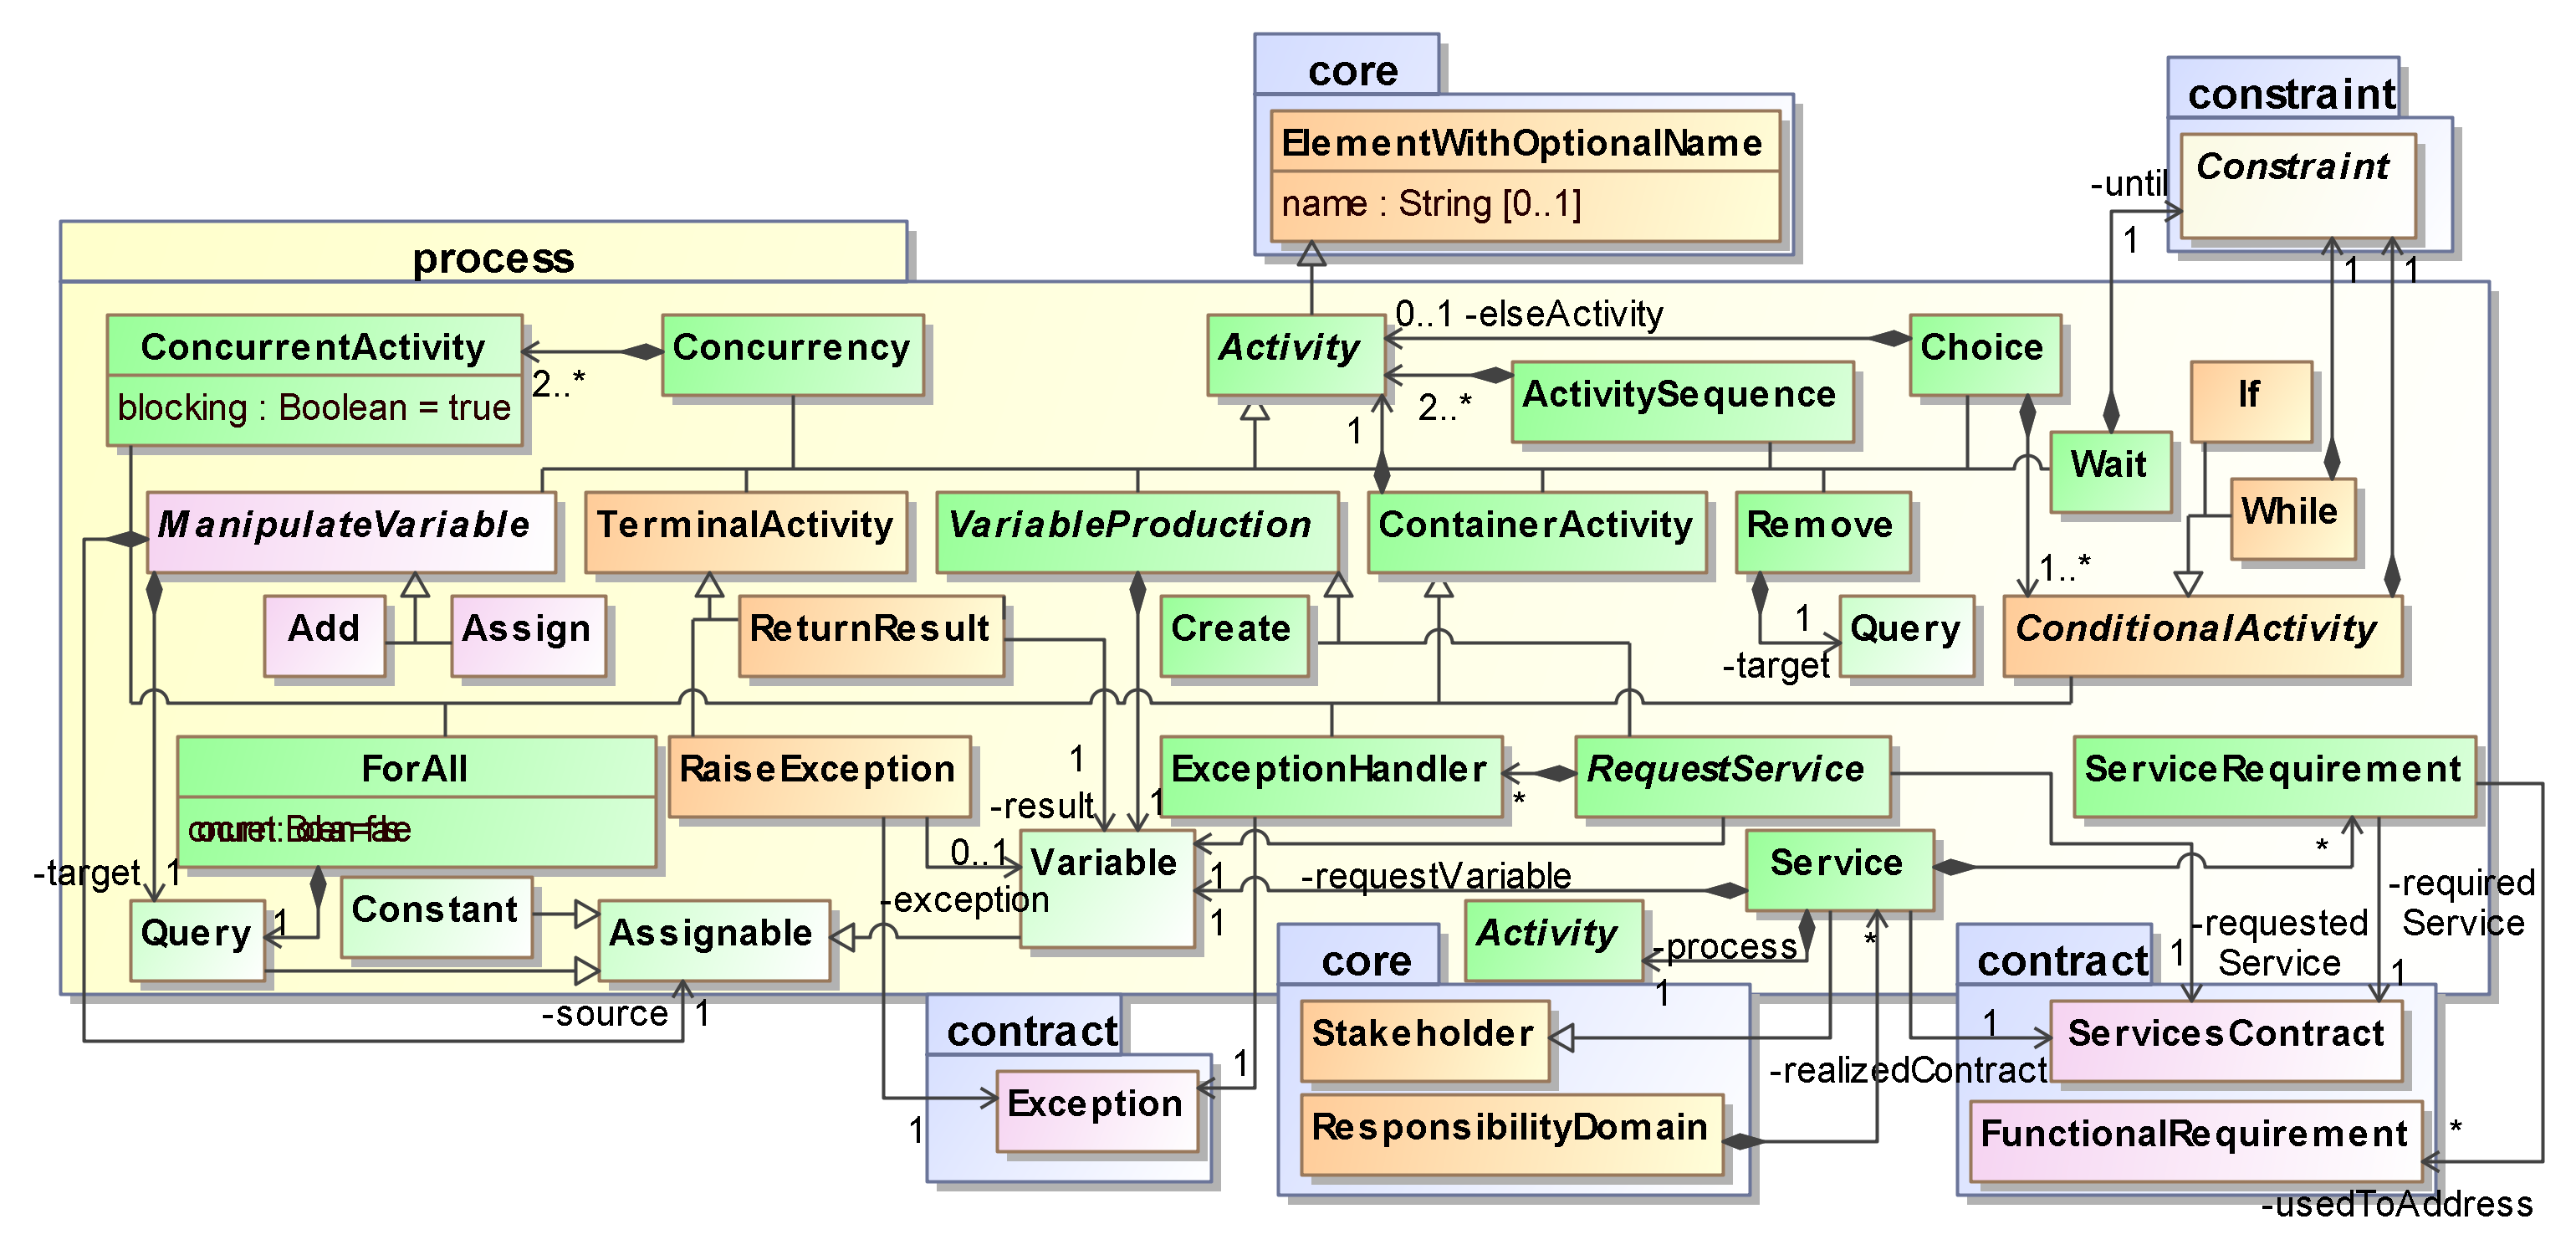
\includegraphics{process}
  \caption{The modeling constructs available for specifying services and processes in URDAD}
  \label{fig:processModule}
\end{figure}

Finally we use URDAD to design its analysis process. For this we use the URDAD modeling constructs for process specification shown in figure \ref{fig:processModule} (of course via the URDAD-DSL text grammar). Note that, following the URDAD process discussed in \ref{sec:urdad} we first specify the services we want to use to address each of the functional requirements (the \verb+usedToAddress+ links between a service requirement and a functional requirement represents the satisfaction links of \cite{ramesh_toward_2001}) before choreographing the process across these services. 

The following listing is an excerpt of the URDAD analysis process generated by applying URDAD to design the \verb+performAnalysis+ service:
\lstset{language=urdad,caption=Specifying the performAnalysis service in the textual URDAD DSL syntax.,label=serviceTextSyntax}
\begin{lstlisting}[numbers=left,escapechar=|]
Service provideServiceImpl realizes provideService receiving Variable provideServiceRequest ofType ProvideServiceRequest
{
  use provideServicesContract toAddress ( serviceContractSpecified serviceHasStakeHolders stakeholderRequirementsConsistent)
  use sourceService toAddress (serviceSourcedFromEnvironment)
  use designService toAddress (serviceSpecified)
        
  Process doSequential
  {
    create Variable provideServiceContractRequest ofType ProvideServiceContractRequest
    set Query OCL:"provideServiceContractRequest.serviceRequirements" equalTo Query OCL:"provideServiceRequest.serviceRequirements"
    requestService provideServiceContract with provideServiceContractRequest yielding Variable provideServiceContractResult ofType ProvideServiceContractResult raises (NoStakeholdersException InconsistentRequirementsException) 

    create Variable sourceServiceRequest ofType SourceServiceRequest
    set Query OCL:"sourceServiceRequest.serviceContract" equalTo Query OCL:"provideServiceContractResult.serviceContract"
    requestService sourceService with sourceServiceRequest yielding Variable sourceServiceResult ofType SourceServiceResult on NoRealizingServiceException
    doSequential
    {
      create Variable designServiceRequest ofType DesignServiceRequest
      set Query OCL:"designServiceRequest.serviceContract" equalTo Query OCL:"provideServiceContractResult.serviceContract"                
      requestService designService with designServiceRequest yielding Variable designServiceResult ofType DesignServiceResult
      forAll requiredService in Query OCL:"designServiceResult.service.requiredServices."
      {
        create Variable provideLowerLevelServiceRequest ofType ProvideServiceRequest
        add Query OCL:"requiredService" to Query OCL:"provideLowerLevelServiceRequest.serviceRequirements"
        requestService provideService with provideLowerLevelServiceRequest yielding variable provideLowerLevelServiceResult ofType ProvideServiceResult 
      } 
    } 
  }             
}
\end{lstlisting}

Comparing the above listing we see that \emph{performAnalysis} process corresponds to the original process discussed in section \ref{sec:urdad}.

  \section{Summary}

\begin{frame}{Summary}
 \begin{itemize}
  \item<+-| alert@+> Different stakeholders in model have overlapping quality requirements.
  \item<+-| alert@+> Process and supporting metamodel has embedded quality drivers.
  \item<+-| alert@+> When using URDAD to design A\&D process, one can regenerate URDAD with its metamodel.
 \end{itemize}
\end{frame}



%\footbibliographystyle{plain}  %%abbrv
%\footbibliography{../../../bibliography}

\end{document}

